%%
%% This is file `sample-sigchi.tex',
%% generated with the docstrip utility.
%%
%% The original source files were:
%%
%% samples.dtx  (with options: `sigchi')
%% 
%% IMPORTANT NOTICE:
%% 
%% For the copyright see the source file.
%% 
%% Any modified versions of this file must be renamed
%% with new filenames distinct from sample-sigchi.tex.
%% 
%% For distribution of the original source see the terms
%% for copying and modification in the file samples.dtx.
%% 
%% This generated file may be distributed as long as the
%% original source files, as listed above, are part of the
%% same distribution. (The sources need not necessarily be
%% in the same archive or directory.)
%%
%% The first command in your LaTeX source must be the \documentclass command.
\documentclass[sigchi]{acmart}

\usepackage{xcolor}
\usepackage{amssymb}
\usepackage{amsmath}
\usepackage{amsthm}
\usepackage{graphicx}

%%
%% \BibTeX command to typeset BibTeX logo in the docs
\AtBeginDocument{%
  \providecommand\BibTeX{{%
    \normalfont B\kern-0.5em{\scshape i\kern-0.25em b}\kern-0.8em\TeX}}}

%% Rights management information.  This information is sent to you
%% when you complete the rights form.  These commands have SAMPLE
%% values in them; it is your responsibility as an author to replace
%% the commands and values with those provided to you when you
%% complete the rights form.
%\setcopyright{acmcopyright}
%\copyrightyear{2018}
%\acmYear{2018}
%\acmDOI{10.1145/1122445.1122456}

%% These commands are for a PROCEEDINGS abstract or paper.
%\acmConference[Woodstock '18]{Woodstock '18: ACM Symposium on Neural
%  Gaze Detection}{June 03--05, 2018}{Woodstock, NY}
%\acmBooktitle{Woodstock '18: ACM Symposium on Neural Gaze Detection,
%  June 03--05, 2018, Woodstock, NY}
%\acmPrice{15.00}
%\acmISBN{978-1-4503-9999-9/18/06}


%%
%% Submission ID.
%% Use this when submitting an article to a sponsored event. You'll
%% receive a unique submission ID from the organizers
%% of the event, and this ID should be used as the parameter to this command.
%%\acmSubmissionID{123-A56-BU3}

%%
%% The majority of ACM publications use numbered citations and
%% references.  The command \citestyle{authoryear} switches to the
%% "author year" style.
%%
%% If you are preparing content for an event
%% sponsored by ACM SIGGRAPH, you must use the "author year" style of
%% citations and references.
%% Uncommenting
%% the next command will enable that style.
%%\citestyle{acmauthoryear}

%%
%% end of the preamble, start of the body of the document source.
\begin{document}

%%
%% The "title" command has an optional parameter,
%% allowing the author to define a "short title" to be used in page headers.
\title{Interactive Visualization of Neural Network Activities}

%%
%% The "author" command and its associated commands are used to define
%% the authors and their affiliations.
%% Of note is the shared affiliation of the first two authors, and the
%% "authornote" and "authornotemark" commands
%% used to denote shared contribution to the research.
\author{Zijian Li}
%\email{trovato@corporation.com}
%\orcid{1234-5678-9012}
%\author{G.K.M. Tobin}
%\authornotemark[1]
%\email{webmaster@marysville-ohio.com}
\affiliation{%
  \institution{University of Washington}
}

\author{Callin Switzer}
\affiliation{%
  \institution{University of Washington}
}

\author{Yue Zhao}
\affiliation{%
  \institution{University of Washington}
}

\author{Zhengde Zhao}
\affiliation{%
  \institution{University of Washington}
}
%%
%% By default, the full list of authors will be used in the page
%% headers. Often, this list is too long, and will overlap
%% other information printed in the page headers. This command allows
%% the author to define a more concise list
%% of authors' names for this purpose.
%\renewcommand{\shortauthors}{Trovato and Tobin, et al.}

%%
%% The abstract is a short summary of the work to be presented in the
%% article.
\begin{abstract}
  This project builds an interactive visualization system for neural networks, with application to the flight modeling of a virtual moth. The system visualizes the weight connections, as well as the activation values of the nodes real-time in response to adjustments in the input values. Weights distribution in the network is shown, with the brushing scheme to select absolute values in the desired range. The graph is plotted using the force directed layout scheme to accommodate to networks with different sizes. Visualization results using different neural network structures are shown with various interaction. Extraction of useful information using the system is discussed with examples.
\end{abstract}

%%
%% The code below is generated by the tool at http://dl.acm.org/ccs.cfm.
%% Please copy and paste the code instead of the example below.
%%

%%
%% Keywords. The author(s) should pick words that accurately describe
%% the work being presented. Separate the keywords with commas.
\keywords{Neural networks, Data Visualization, Interactive}

%%
%% This command processes the author and affiliation and title
%% information and builds the first part of the formatted document.
\maketitle

\section{Introduction}

\subsection{Background}

%% The primary parameter given to the ``\verb|acmart|'' document class is the {\itshape template style} which corresponds to the kind of publication or SIG publishing the work. This parameter is enclosed in square brackets and is a part of the {\verb|documentclass|} command:
%%\begin{verbatim}
%%  \documentclass[STYLE]{acmart}
%%\end{verbatim}

%%Journals use one of three template styles. All but three ACM journals use the {\verb|acmsmall|} template style:
%%\begin{itemize}
%%\item {\verb|acmsmall|}: The default journal template style.
%%\item {\verb|acmlarge|}: Used by JOCCH and TAP.
%%\item {\verb|acmtog|}: Used by TOG.
%%\end{itemize}

%%The majority of conference proceedings documentation will use the {\verb|acmconf|} template style.
%%\begin{itemize}
%%\item {\verb|acmconf|}: The default proceedings template style.
%%\item{\verb|sigchi|}: Used for SIGCHI conference articles.
%%\item{\verb|sigchi-a|}: Used for SIGCHI ``Extended Abstract'' articles.
%%\item{\verb|sigplan|}: Used for SIGPLAN conference articles.
%%\end{itemize}

Insects like moths have very simple brains, yet they are capable of precise and subtle flying maneuvers, which involve complex fluid dynamics. They generate locomotor force by activating the flight muscles to move their wings, and the aerodynamic forces and torques it generates enable they to preform various flying behaviors including fast forward, odor plume tracking, hovering in front of flowers, decelerating upon approach and conpensating for enrionmental perturbations \cite{Stevenson1665}  \cite{Willis1991}
. To understand how moths control their flight is already by itself interesting, not to mention that  bio-inspired flapping wings system has potential application to micro air vehicles according to Chen in \cite{Chen_2018}. 

Multiple recent researchers has targeted this question. In \cite{Hedrick3114}, the authors treated this question as an inverse problem, where the input of the system is the initial position, initial velocity, targeting position and targeting velocity while the output of the system is the wing motion. They developed an aerodynamic model illustrating how a particular motion in the wings of a moth could result in a kinetic motion. In \cite{Dyhr1523}, they found that not only the wings but also the shape of the body plays an important role in a moth's flight control. New variables such as the angle of the body of the moth were introduced into the model. Further study has also shown that structural deformation also affects flapping wing energetics, see \citep{Jankauski_2018}. Nevertheless, to solve the inverse problem of flight control is intrinsically difficult. It involves solving a highly nonlinear dynamically system. 

\subsection{Project Goal}
In the related study by Dr. Switzer, a researcher in the Biology Department of University of Washington, several deep neural networks are designed to solve the moth flight control problem. Imagine a moth trying to fly, it knows its current position and state, and where it wants to go. To achieve the goal, it needs to figure out the force control over its body that takes it on the trajectory to the destination, ending up with some final velocity. The feedforward neural networks were designed going from "where I am" and "where I want to go" (inputs), to the corresponding controls and final derivatives (outputs). The neural networks are trained with artificial dataset from Monte Carlo simulation, and are pruned to regularize the weights. 

The goal of this project is to visualize the architectures of the pruned neural networks, which is capable of eliminating weights close to zero. Moreover, this project is unique in that it also interactively show the values of the nodes, in response to real-time adjustment of the input values.

\subsection{Related Work}
Neural networks are a special type of graphs, which are highly organized in their structures. For a feedforward neural network used in this study, nodes in the graph are divided into layers, and the group of nodes in each layer only connect with nodes in adjacent layers. \cite{bischof1992visualization} described the visualization of feedforward neural networks, which aligns the position of the nodes according to their layer number. Figure \ref{ffnn} shows the structure of a fully-connected feedforward neural network used in the virtual moth modeling, in a typical way of conceptually visualizing a neural network.  
\begin{figure}[h]
  \centering
  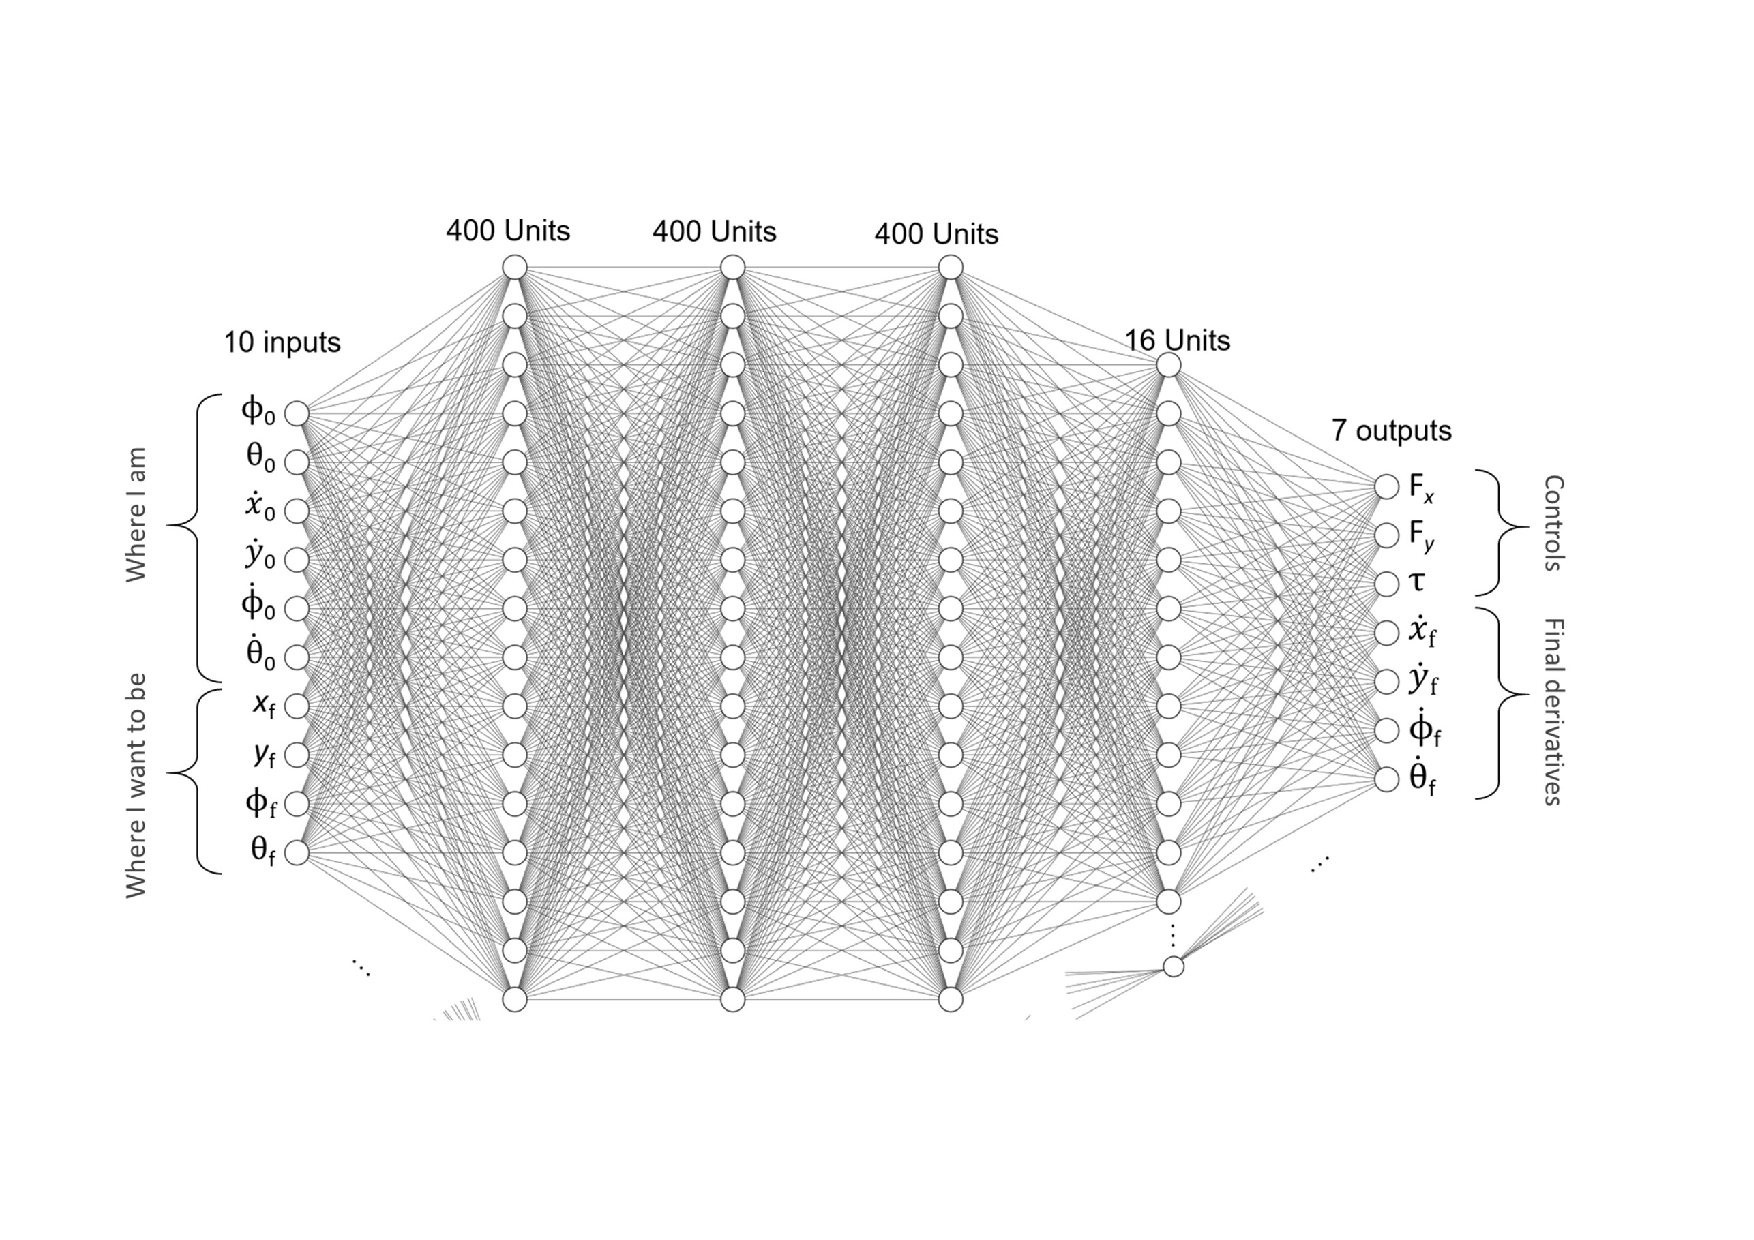
\includegraphics[width=\linewidth]{ffnn.pdf}
  \caption{Feedforward Neural Network}
  \Description{Example of a fully-connected feedforward neural network used in the modeling of a virtual moth.} 
  \label{ffnn}
\end{figure}

The above graph is clear in understanding the model structure conceptually, but has some drawbacks. First of all, this visualization does not show information such as activation values on the nodes and the weights of the connections. Secondly, it is bad under scaling. For example, there are 400 units in the middle layers, but the plot is incapable of showing the complete weight structure. Lastly, the layout is only suitable for simple structures like feedforward network. With the rapid development of new network structures nowadays such as the recurrent neural network \cite{rumelhart1988learning}, we need a more flexible framework to visualize neural networks.

\section{Methods}
\subsection{Computational Graph Construction}
A fully-connected feedforward neural network has connections between each two adjacent layers in the form of a bipartite graph, which can be represented by a weight matrix $W$, where $W_{ij}$ goes from the $i$-th node in the previous layer to the $j$-th node in the next layer. The weight matrices are also the typical data structure of storing a neural network. From the weight data, we can construct a directed graph 
\[
G = (V, E)
\]
consisting of the set of nodes $V$ and the set of edges $E$. The elements in the graph have the following properties:
\begin{align*}
& v \in V: \ \mbox{node ID}\ i, \ \mbox{layer number}\ l, \ \mbox{activation value}\ u, \\
& e \in E: \ \mbox{source}\ i, \ \mbox{target}\ j, \ \mbox{weight}\ w.
\end{align*}

Note that the activation value $u$ on each nodes is determined not only by the neural network itself, but also depends on the input values. Therefore, the network construction should be real-time in response to interactive input selection. To solve this problem, we construct the graph together with all the element properties. For the feedforward neural networks in our study, we implement the forward pass algorithm starting from the input layer values $u^{(0)}$., and iterates throughout the whole network to the output layer:
\[
u^{(l+1)}_j = \tanh \left(\sum_{i} W^{(l+1)}_{i,j} u^{(l)}_i + b^{(l+1)_j\right).
\]

Since many neural networks are highly pruned in our study, a large portion of weights are zeros or close to zero. It is undesirable to show these edges, and thus we throw away them in the construction phase to reduce the amount of computation in the following visualization stage. Nodes that are not connected to any edge are also thrown away after edge trimming to keep the graph connected.

\subsection{Force Directed Layout}
In stead of aligning the nodes according to the layers into strict lines, we use the force directed layout scheme \cite{fruchterman1991graph}. Each node $v_i$ is regarded as a charged particle with charge $q_i$. Each two nodes $v_i$ and $v_j$ repel each other with the force
\[
F = \frac{q_i q_j}{d_{ij}^2}.
\]
Each edge $e_{ij}$ is considered as a spring, applying the attracting force to the nodes it connects:
\[
F = k(L - d_{ij}).
\]
Besides, each node in motion is subject to air resistance
\[
F = -b v_i.
\]
At each time step, the forces acting on each node are calculated, which are then integrated to update its velocity and position. In our system, we implement the force directed layout scheme with d3-force, which uses a velocity Verlet numerical integrator for simulating physical forces on particles. 

To show the layered structure of the neural network, we apply customized external force field. Similar to plotting nodes in different layers onto different X-positions, we apply attractive X-forces towards different X-position for nodes in different layers. A constant attractive force in the Y direction is also applied to ensure the vertical symmetry of the network. The whole graph is also attracted to the center of the plot. The charges and forced are chosen according to the total number of nodes in the graph:
\[
F_X \sim \frac{1}{|V|^2}, \quad q \sim \frac{1}{|V|}.
\]

\subsection{Visual Encoding}
Once the graph of the neural network is constructed, we can encode the properties of the nodes and edges. The layer numbers of the nodes are encoded with the customized force directed layout. To represent the activation values of the nodes and highlight the nodes with the largest absolute values, we use the sizes of the nodes to encode the absolute values. The sign of the activation values are encoded with two different colors, representing positive and negative. Since the activation function in the neural network always scales the values of the nodes to $[-1,1]$, we can control the size of the nodes in a certain range. For input and output layers where the activation function is not applied, additional scaling scheme (e.g. activation function) can be applied to adjust the size.

To highlight the most important weights and not to be distracted by other edges, we use both thickness and opacity to over-encode the absolute values of the weights. Since the network is fully-connected between layers with upto 800000 edges, such over-encoding can avoid small weights to cover the space and highlight the dominant weights. To make the system adjustable to different networks, the encoding is linearly scaled according to the maximal weight.

\subsection{Interaction}
The key feature of the interactive neural network visualization system is the automatic changing of node sizes in response to adjusting input values. For the 10 input values of the virtual moth model, we use slide bars for the user to adjust these values. The activation values of all the nodes in the network are computed in real-time and visualized on the plot. The values in the input layer are also visualized in the X-positions on the slide bar, with values shown in text.

Another important interaction is the brushing scheme to select weights with absolute values in a desirable range. For each edge, we plot its absolute weight on the brushing bar. The sign of the weight is encoded with the color and the Y-position on the brushing bar, forming two lines of dots in two distinct colors. From the brushing bar, the user can see the distribution of the weights in the neural network from the dot density. The "absolute value + double lines" design can exclude the middle part of weights around zeros in a simple way.

In addition to the above two major interactions, the visualization system also allows for other interactions. We use tooltips for detailed information demand, for example the layer number $l$ and activation value $u$ of a node, and the connection information and weight value of an edge. The drag-and-move interaction provided by the force directed layout is also useful. As all the nodes in a single layer (except the input and output layer) are essentially equivalent to each other, the positions of them are arbitrary. User can drag nodes to avoid overlapping of the main edges. Besides, there is a drop-down menu for users to choose the neural network models to visualize. For the virtual moth study, we provide 6 feedforward networks with different structures.

\section{Results}
\subsection{Visualization Interface}
Figure \ref{inter} shows the interface of the web-based interactive neural network visualization system. Users can use the drop-down menu to load the neural network model to visualize. The force directed scheme then configures the layout of the graph plot. By adjusting the slide bars on the left, users can see the activation value change of all the nodes instantly, encoded by the size of the nodes. Users can use the brushing bar at the bottom to choose the absolute value range. The brushing bar also shows the weight distribution, as well as how many weights are selected in the target range.

\begin{figure}[h]
  \centering
  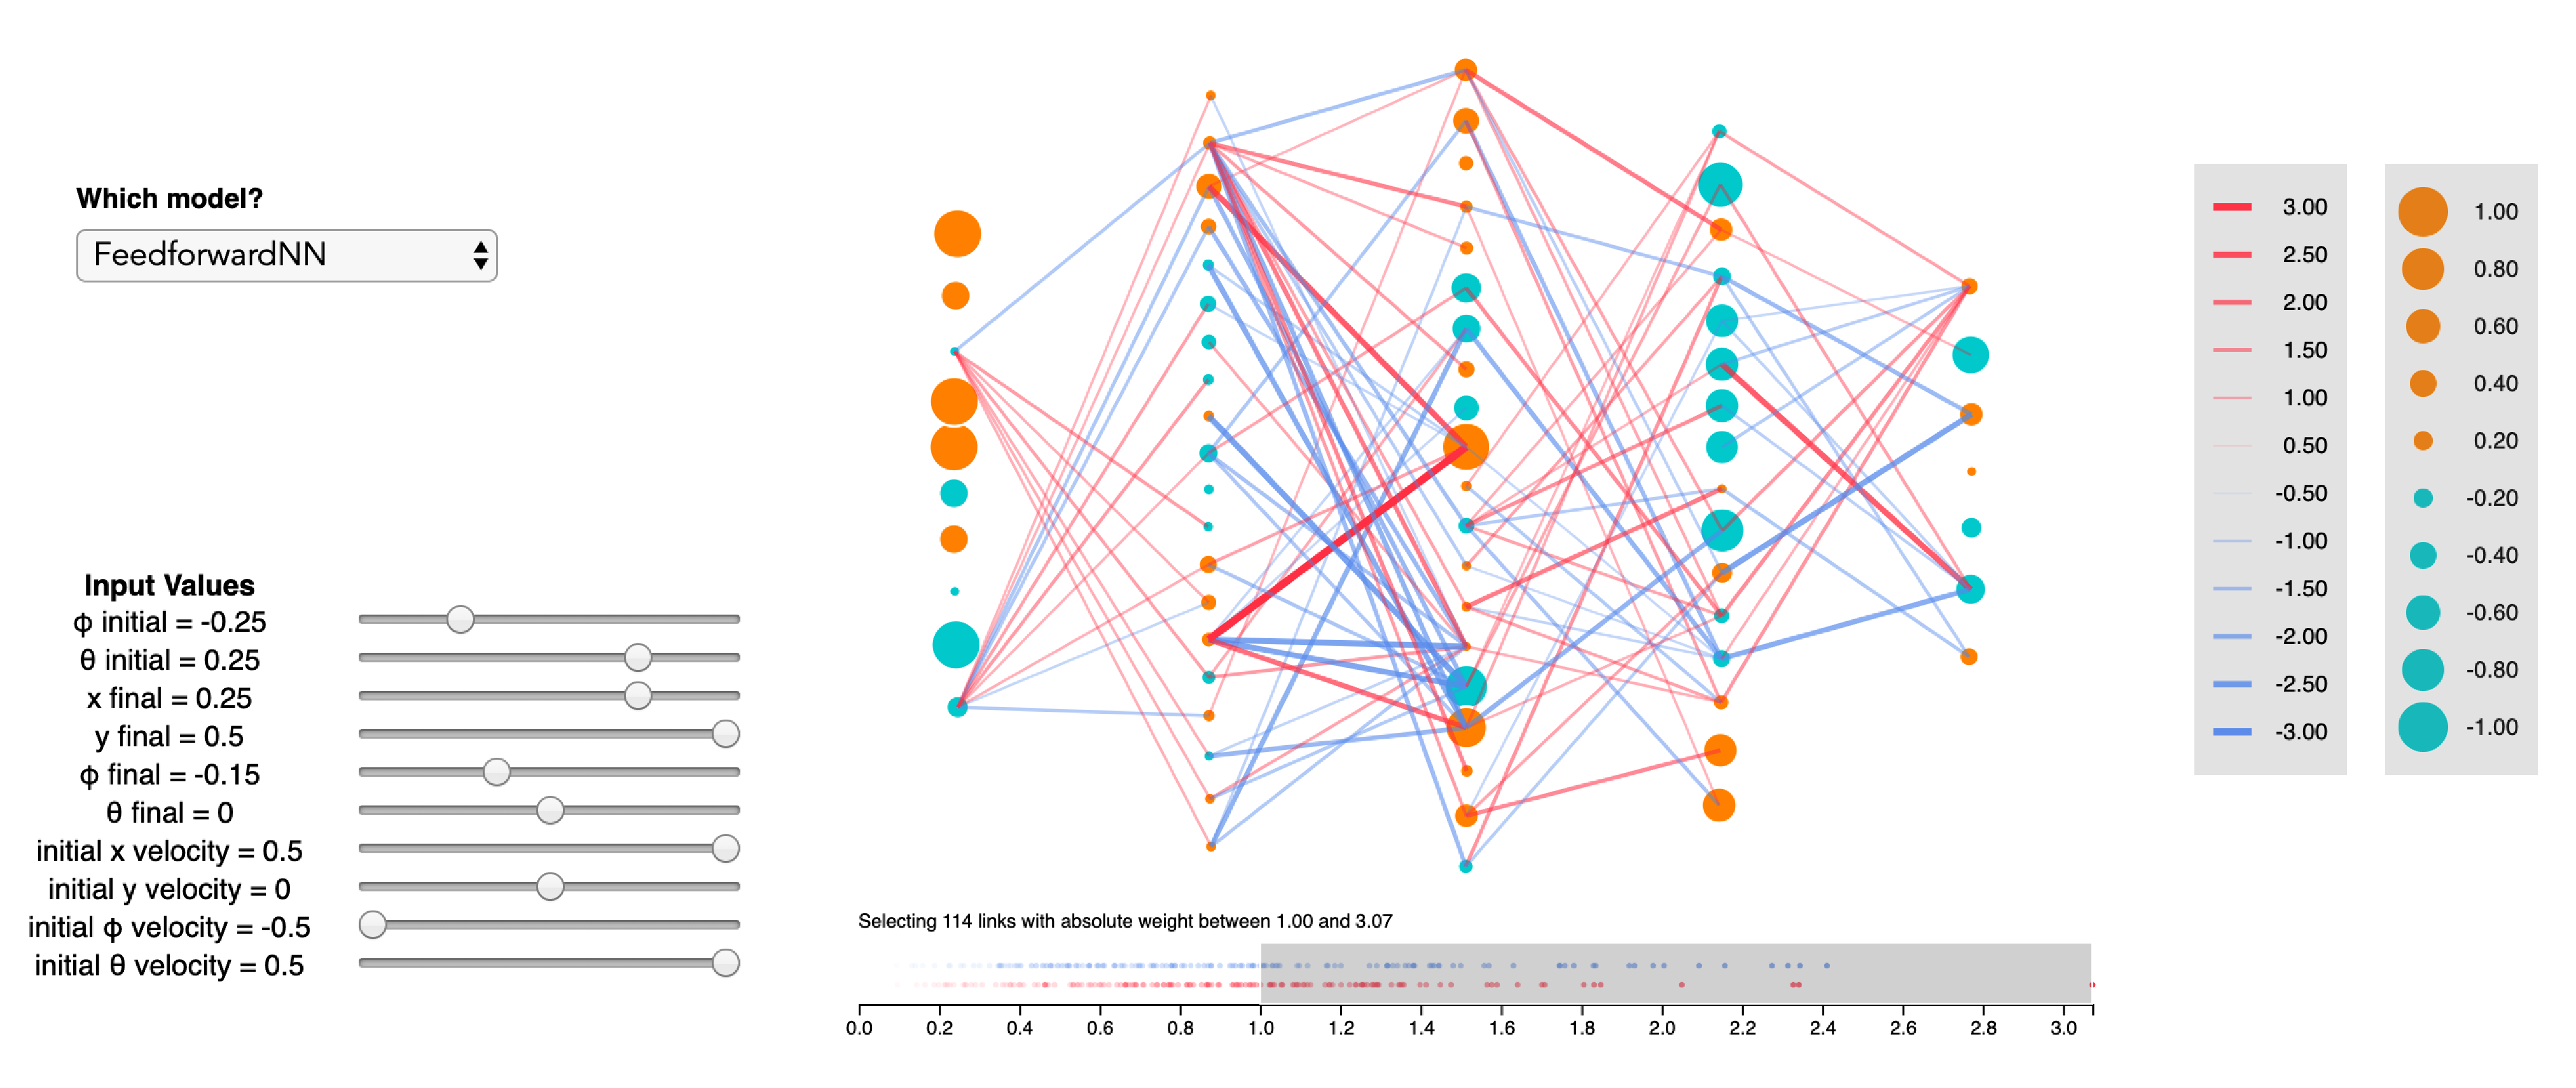
\includegraphics[width=\linewidth]{interface.pdf}
  \caption{Visualization Interface}
  \Description{The web-based interface of the interactive neural network visualization system.}
  \label{inter}
\end{figure}

As a base example of our visualization, we use the above pruned neural network with $3$ hidden layers of sizes: $(20, 20, 16)$. Input values are chosen using the slide bars to mimic a jumping up of the virtual moth: $x_f = 0.25, y_f = 0.5, \dot{x}_0 = 0.5, \dot{y}_0 = 0, \phi_0=-0.25, \theta_0=0.25, \phi_f=-0.15, \theta_f=0, \dot{\phi}_0 = -0.5, \dot{\theta}_0 = 0.5$. The brushing bar selects only weights with absolute values over 1. We can see that the network is sparse under weight filtering, and there are several dominant edges with large weight values. For the nodes, the visualization shows that only a subset of nodes have significant activation values, and many of them are zeros or close to zero. The weight distribution is shown in the brushing bar, indicating the network is pruned to exclude weights close to zero. 

\subsection{Scaling to Large Networks}
The visualization system is capable to accommodate large neural networks as well. Figure \ref{max} shows the visualization of a neural network with hidden layer sizes: $( 512, 512, 512, 512)$. Comparing to the previous example, the network is larger in both depth and width, with over 2000 nodes and nearly 800000 edges. We can see that the force directed layout fits this huge network in the plot space nicely. The layers are represented as the disk-shaped clusters. Computational wise, the largest neural network in our study only takes seconds to load and configure the layout, which is tolerable.

\begin{figure}[h]
  \centering
  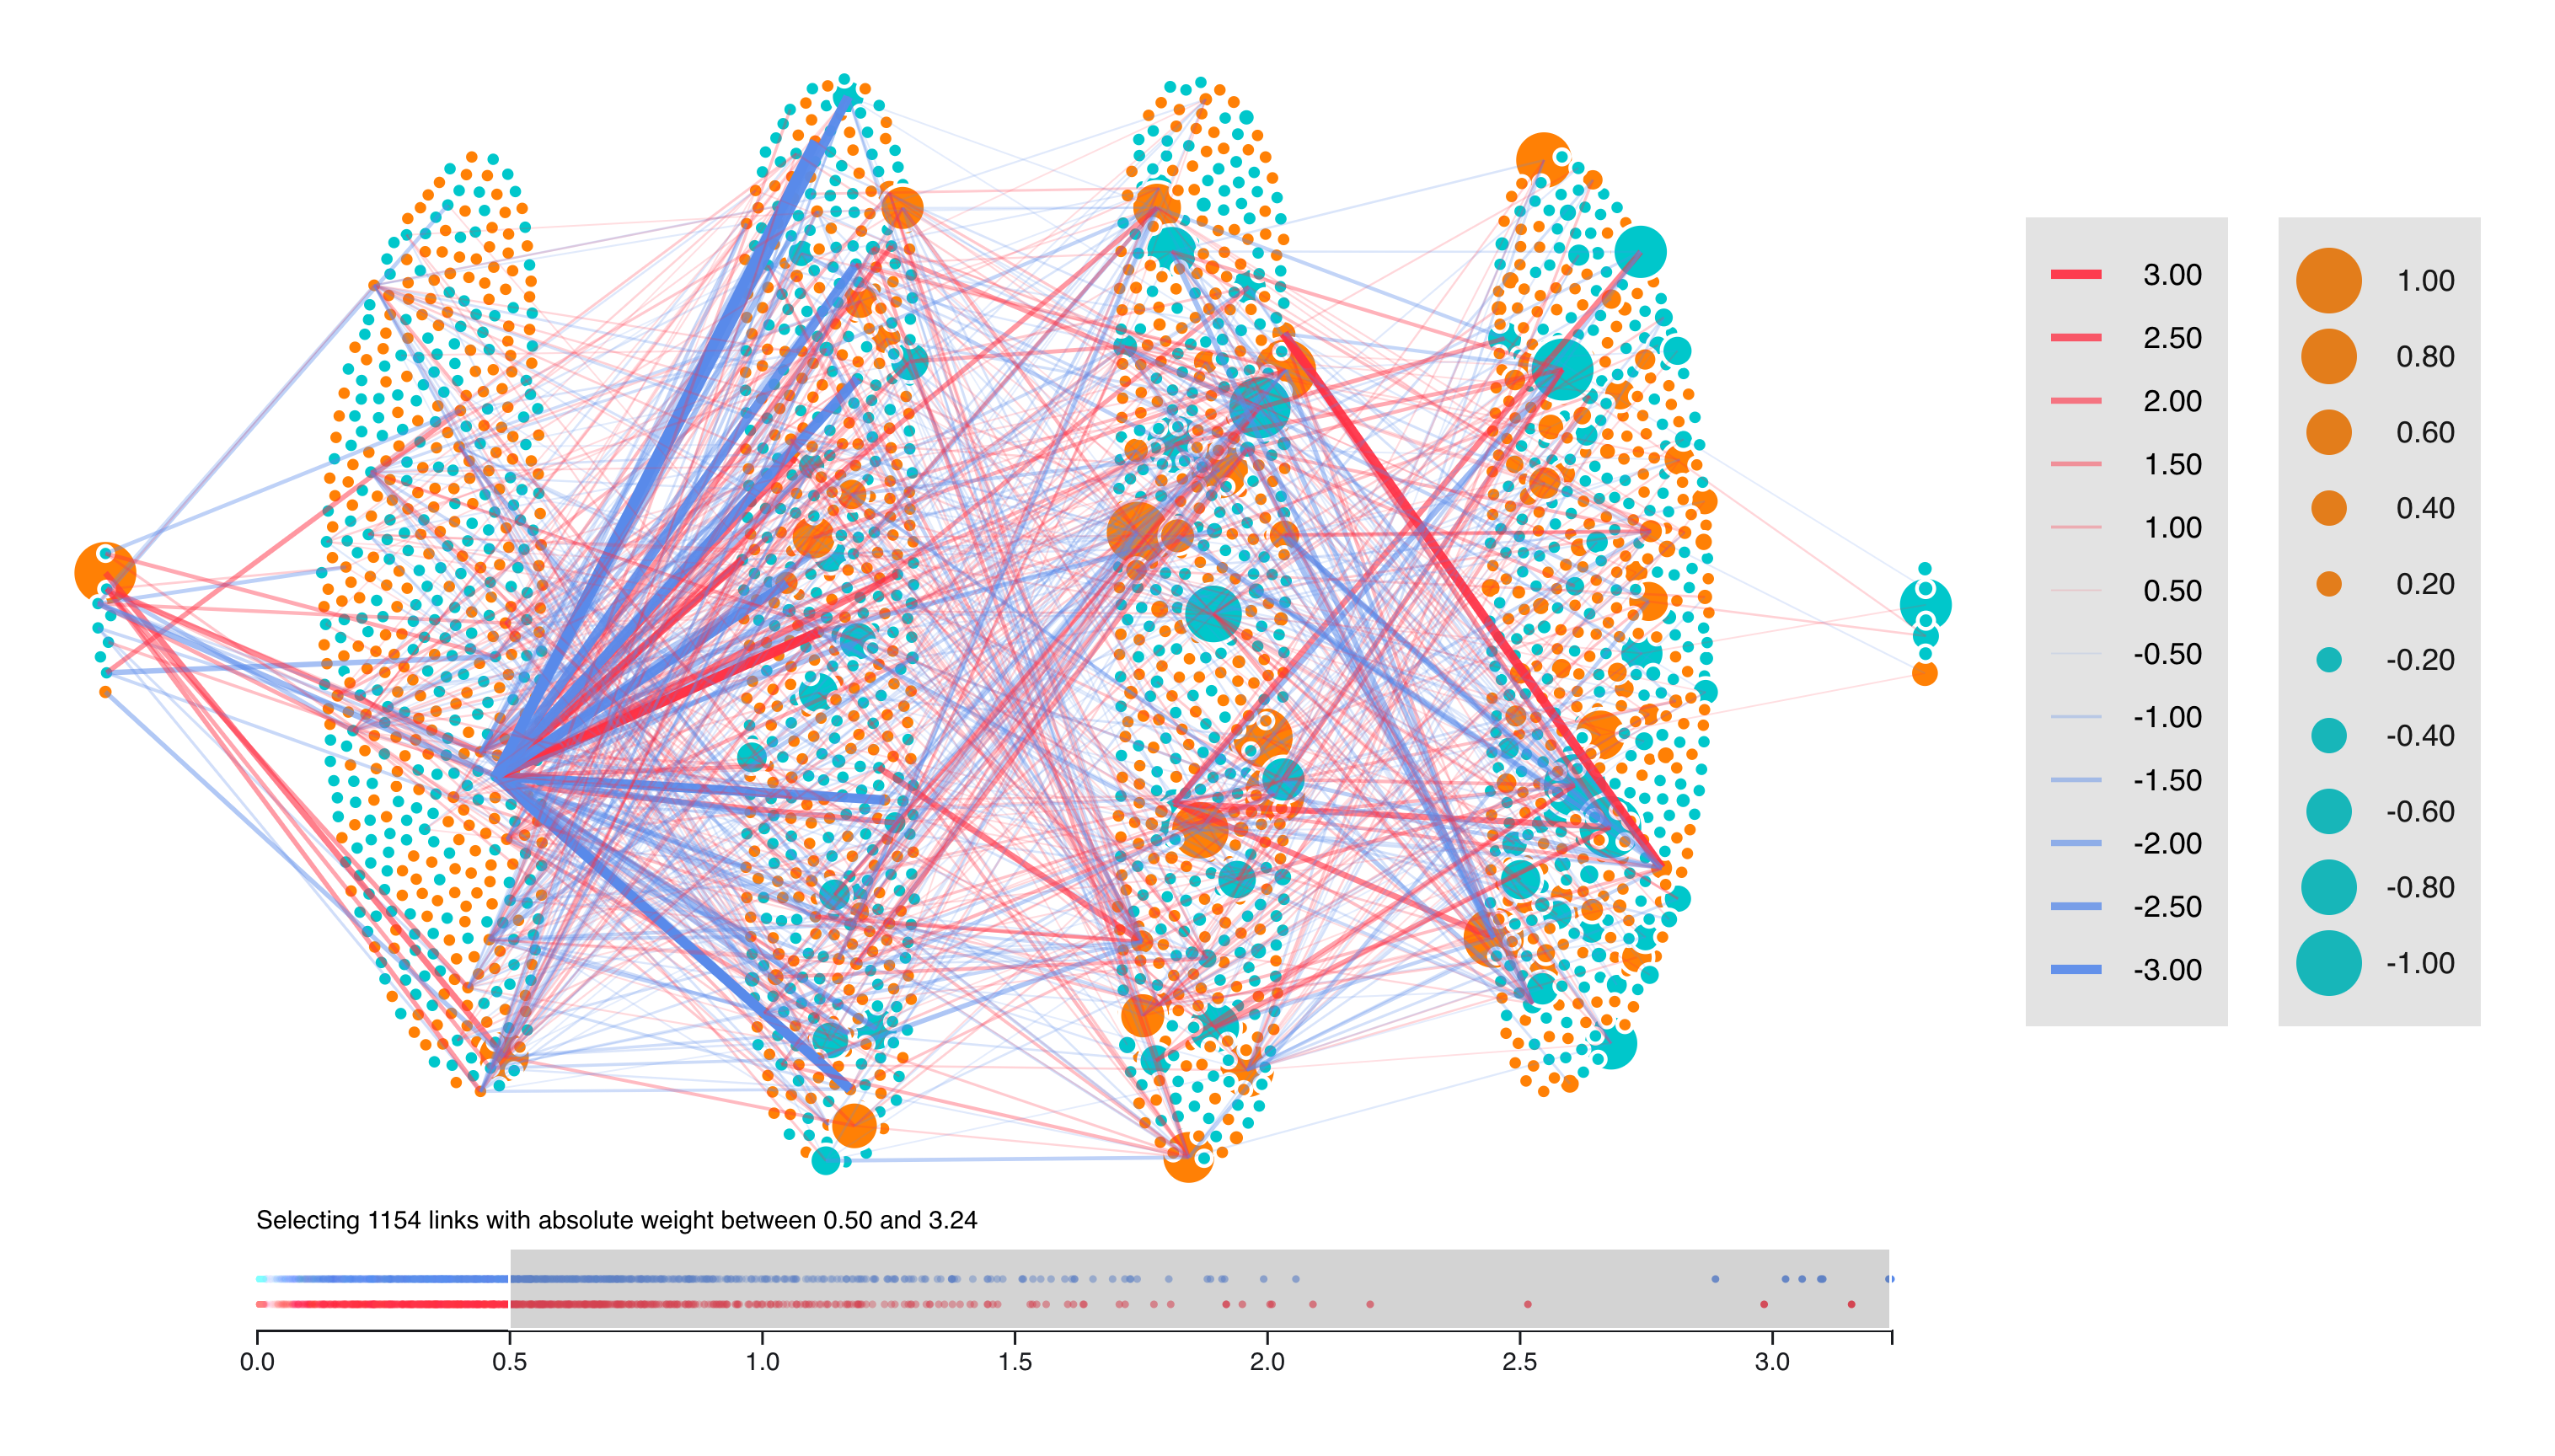
\includegraphics[width=\linewidth]{NNmax1.png}
  \caption{Large Neural Networks}
  \Description{The visualization system is capable of accommodating to large neural networks automatically.}
  \label{max}
\end{figure}

\section{Discussion}
The interactive neural network visualization system provides useful information to users in both training and analysis stages. By using the brushing bar to exclude weights close to zeros, the user can get an idea of how the network can be trimmed. For example, in Figure \ref{inter}, we can see that the network is sparse under weight filtering, and there are several dominant edges with large weight values. The weight distribution shows that the absolute values of the weight distribution is dense around 1, indicating that the network has been pruned to exclude weights close to zero. For the large network example in Figure \ref{max}, we can see there are areas where the most of the largest weights are going out, indicating the hot spots in the neural network. \\

The interaction of adjusting input values is also useful in understanding the neural network, and is helpful for a explainable model. In Figure \ref{adjust}, we show two scenarios with the same inputs as in Figure \ref{inter}. The only difference is that in the bottom plot $y_f$ is adjusted from $0.5$ to $-0.5$. We can see that a different group of nodes are in active now, and some nodes have a sign change. Researchers can use this feature to identify the active area in the neural network while doing certain movement, and which nodes are interconnected. 

\begin{figure}[h]
  \centering
  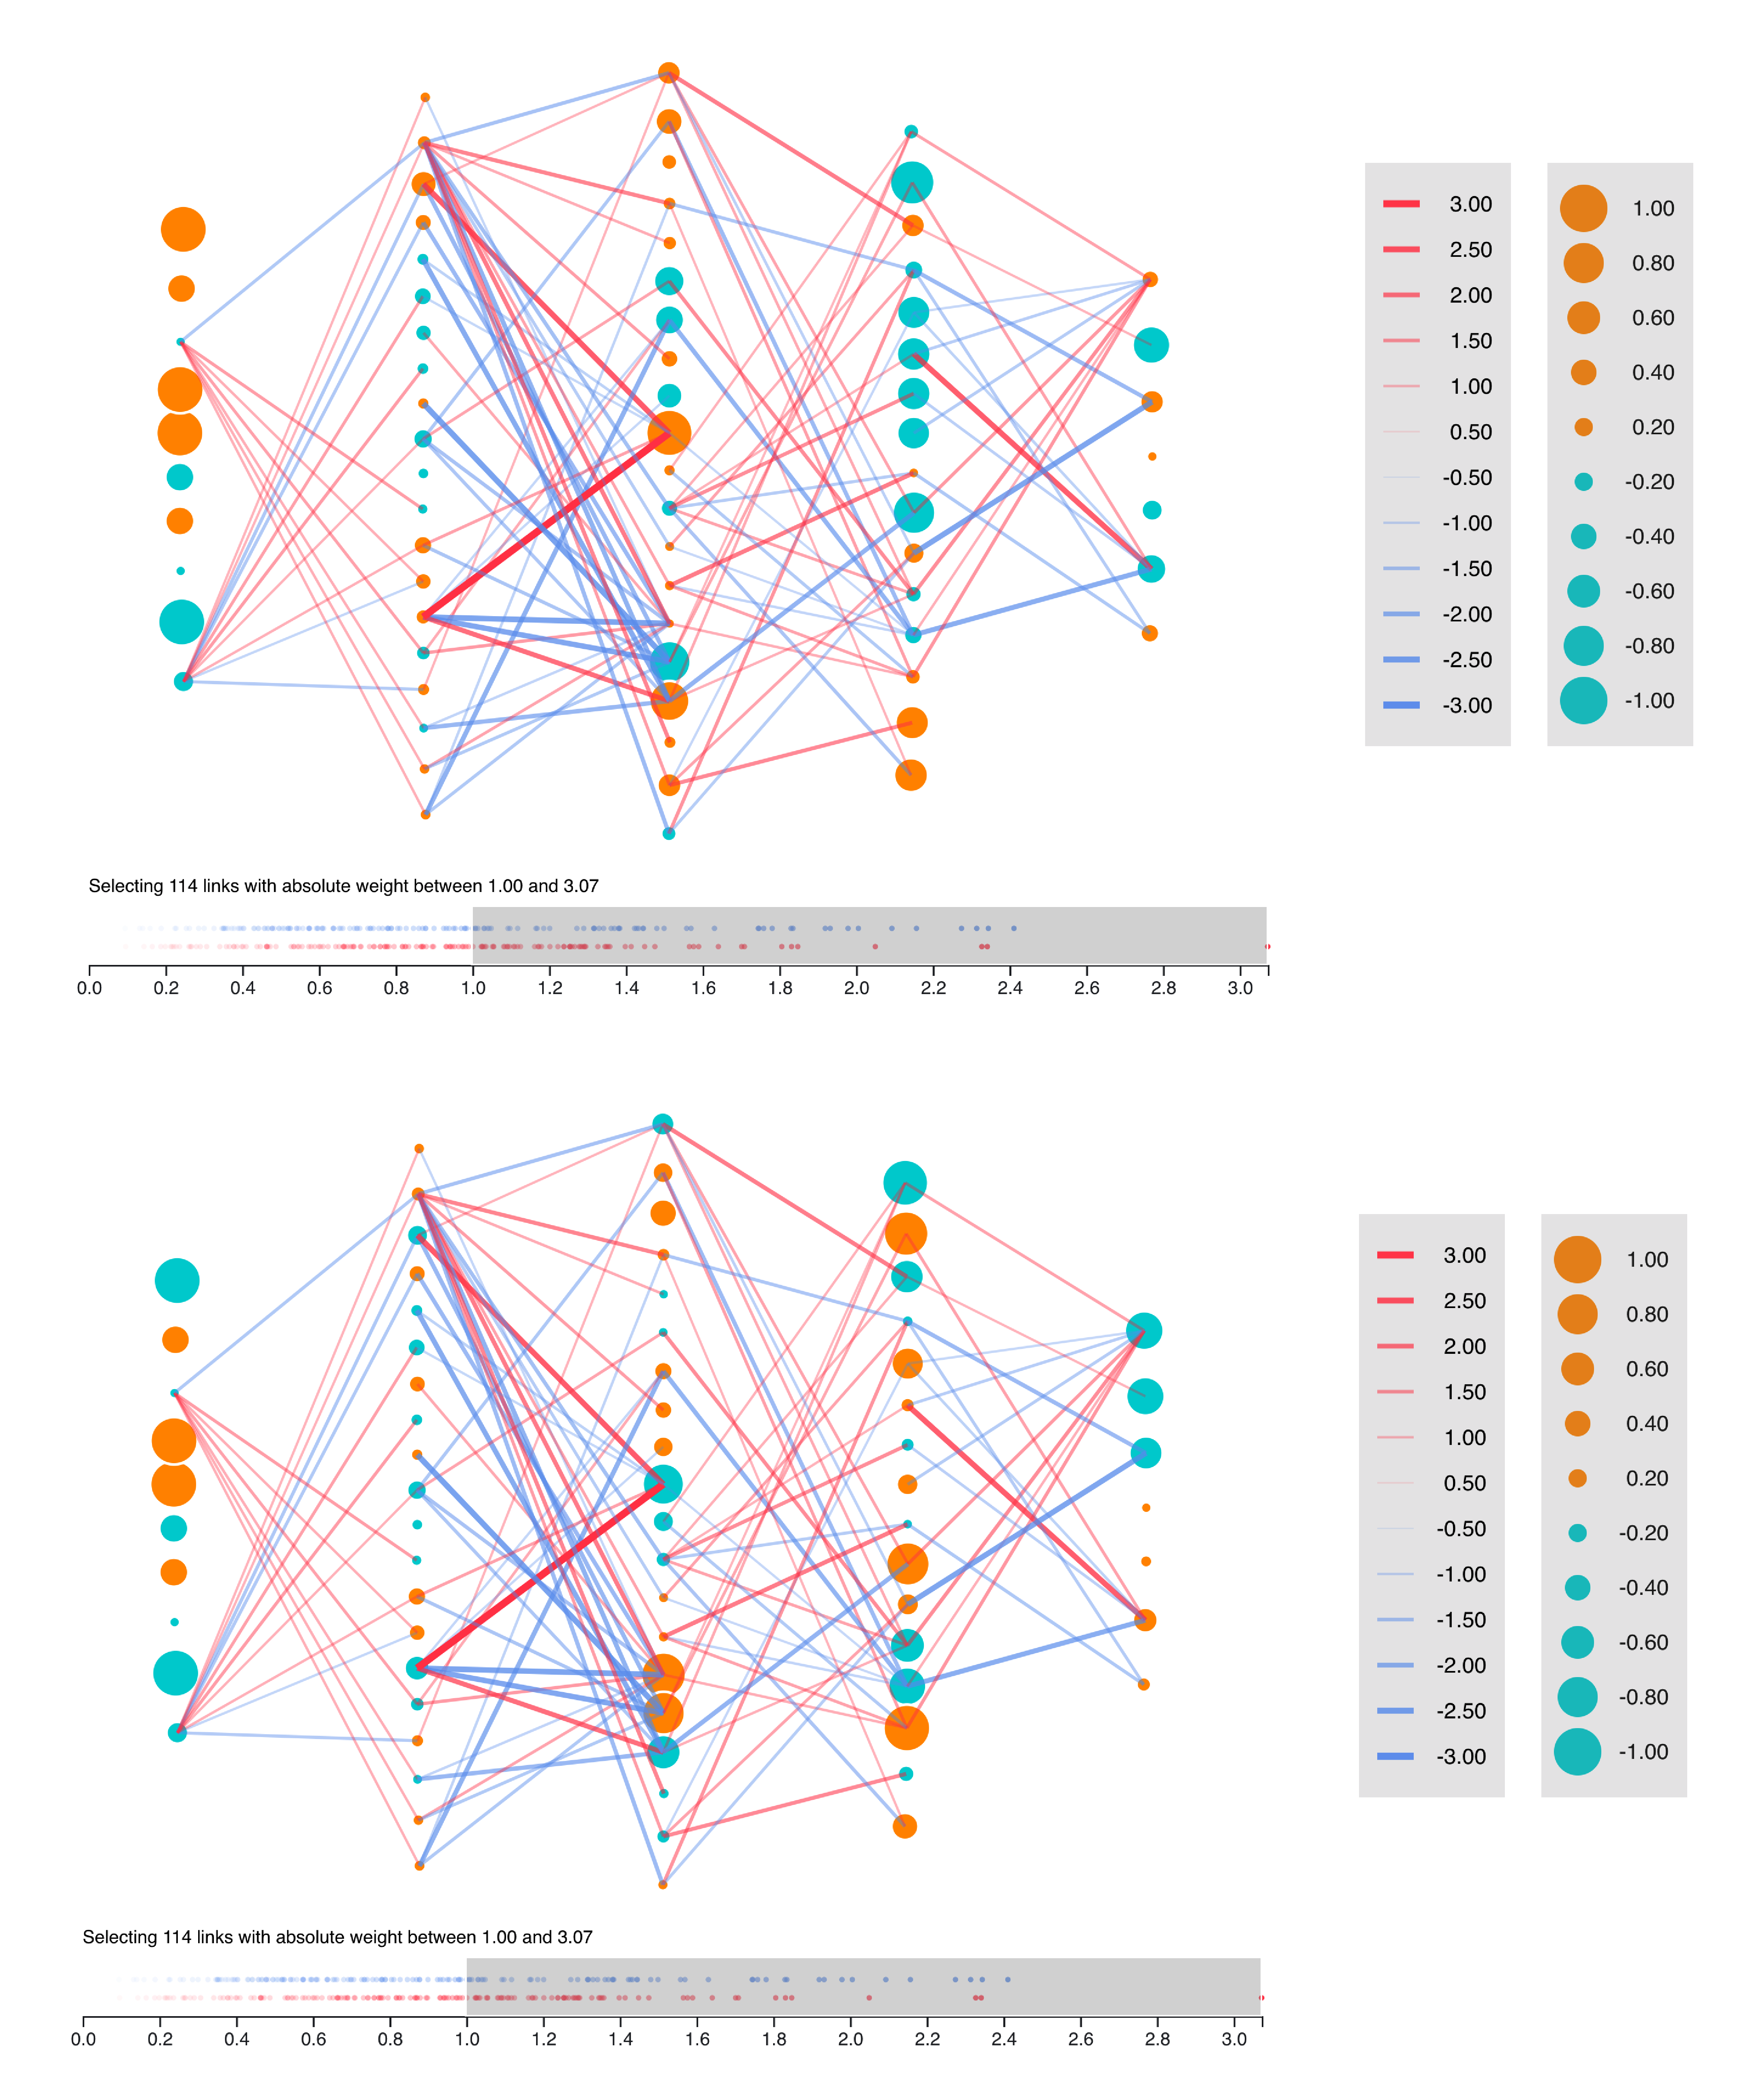
\includegraphics[width=\linewidth]{compare.pdf}
  \caption{Input Adjustment}
  \Description{Comparing the node values under adjustment of a single input value.}
  \label{adjust}
\end{figure}

\section{Future Work}
Besides the current features, there can be additional improvements in future work. The in addition to changing the node values in real-time, we can also change the network structure at the same time. Nodes that are of zeros activation values are of no use in propagating information, thus the edges going out of it are actually useless, regardless of their large weights. Therefore, we may define the activity level of each edge by the activation level of the outgoing node. The visualization of the activity level can be encoded such that inactive edges are invisible (e.g. use thickness or opacity).

Additionally, we may show the strongest path that is connected to each node upon tooltip. Also, it is interesting to visualize the configuration of the virtual moth in real-time (imaging a moth that moves its body), which helps the audience to understand the meaning of the inputs and outputs better. Lastly, we can visualize the distribution of the node values in real-time, as an estimation of "neuron activity level".
\end{itemize}


%\section{Rights Information}
%
%Authors of any work published by ACM will need to complete a rights
%form. Depending on the kind of work, and the rights management choice
%made by the author, this may be copyright transfer, permission,
%license, or an OA (open access) agreement.
%
%Regardless of the rights management choice, the author will receive a
%copy of the completed rights form once it has been submitted. This
%form contains \LaTeX\ commands that must be copied into the source
%document. When the document source is compiled, these commands and
%their parameters add formatted text to several areas of the final
%document:
%\begin{itemize}
%\item the ``ACM Reference Format'' text on the first page.
%\item the ``rights management'' text on the first page.
%\item the conference information in the page header(s).
%\end{itemize}
%
%Rights information is unique to the work; if you are preparing several
%works for an event, make sure to use the correct set of commands with
%each of the works.




%%
%% The next two lines define the bibliography style to be used, and
%% the bibliography file.
\bibliographystyle{ACM-Reference-Format}
\bibliography{bib}

%%
%% If your work has an appendix, this is the place to put it.
\appendix


\end{document}
\endinput
